% Author: Maxwell Chen
% Email: maxhchen@berkeley.edu

\qns{Filter Design}

Suppose you have been hired to design a biomedical sensor that can detect and output recordings of Alpha brainwaves in the frequency range $8 \, \text{Hz}$ to $13 \, \text{Hz}$. 
Unfortunately, our sensor is faulty: it is also picking up Gamma brainwaves in the frequency range $32 \, \text{Hz}$ to $100 \, \text{Hz}$, interfering with our ability to get clean recordings of alpha brainwaves. 
We want to create a new design for our sensor that can remove this interference, giving us a clearer signal.

\begin{enumerate}
  \qitem What kind of filter could you use to remove this interference? 
  
  \sol { 
  We should use a low-pass filter. The interference is at a higher frequency than our desired signal, so we filter out the higher frequencies and keep the lower frequencies.
  }
  
  \qitem Assume we only have access to resistors and capacitors. \textbf{Sketch the corresponding filter circuit and write out its transfer function.} 

  \sol {
  $$H(j \omega) = \frac{\widetilde{Z}_{out}}{\widetilde{Z}_{in}} = \frac{\frac{1}{j\omega C}}{R + \frac{1}{j \omega C}} = \frac{1}{1 + j\omega RC} = \frac{1}{1 + j \frac{\omega}{\omega_{c}}}$$.

  \begin{center}
  \begin{circuitikz} \draw
    (0, 0) node[ground] {}
      to [sV, l_=$V_{in}$] (0, 4)
      to [R = R] (4, 4)
      to [C = C] (4, 0)
      node[ground] {}

    (4, 3) to[short, -o] (6, 3) node[anchor=west] (A) {A}

    (4, 1) to[short, -o] (6, 1) node[anchor=west] (B) {B}

    (A) to[open, l^=$V_{out}$] (B)
  ;\end{circuitikz}
\end{center}

  }   

  \qitem $\omega_{c} = \frac{1}{RC}$ is the cutoff frequency which determines the frequency at which our filter starts attenuating the signal. \textbf{Should we maximize or minimize $\omega_{c}$ to remove as much of the interference as possible?}

  \sol {
  We should minimize the cutoff frequency. The transfer function will start filtering frequencies sooner, meaning that we maximize the amount by which higher frequencies are attenuated.
  }

  \qitem Say we can set our cutoff frequency to $10 \, \text{Hz}$, $20 \, \text{Hz}$, $32 \, \text{Hz}$, $100 \, \text{Hz}$, or $120 \, \text{Hz}$. Which is the best cutoff frequency, and why?

  \sol {
  20Hz. This is the lowest cutoff frequency we can choose; the Gamma brainwaves will be attenuated more if we choose 20Hz than 32Hz because the transfer function will start filtering at a lower frequency. 10Hz is too low and risks cutting off Alpha brainwaves.
  }   

  \qitem We only have a 3.3 k$\Omega$ resistor in our workstation. What capacitor value should we use for our filter?

  \sol {
  If we want a cutoff frquency of 20Hz, then $f = \frac{\omega_{c}}{2 \pi} = \frac{1}{2 \pi RC} = 20Hz$. So, $C = \frac{1}{2 \pi \cdot 33 \cdot 10^{3} \Omega \cdot 20Hz} = 2.41 \, \mu$F.
  }   

  \qitem Draw the Bode plot for the magnitude and phase response of this filter.

  \sol {
  \begin{figure}[h]
  \centering
  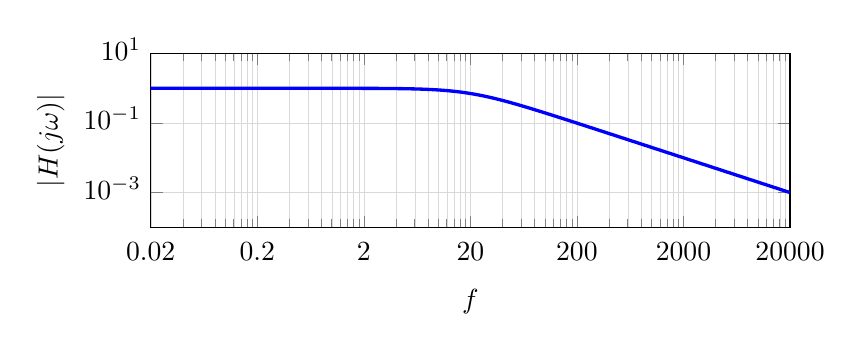
\begin{tikzpicture}[
    declare function={
      mag(\omega)= 1 / sqrt(1 + (\omega / 10^8)^2)
      % Straight line bode approximation
      % mag(\omega)= (\omega < 10^8) * (1) +
      %           (\omega >= 10^8) * (10^8 / \omega)
     ;
    }
  ]
    \begin{loglogaxis}[
      typeset ticklabels with strut,
      ymin=0.0001, ymax=10, ylabel=$|H(j \omega)|$,
      xmin=10^5, xmax=10^11, xlabel=$f$,
      xticklabels={$0.02$,$0.2$,$2$,$20$,$200$, $2000$, $20000$},
      domain=10^5:10^11,
      grid=both, grid style={line width=.1pt, draw=gray!30},
      width=\textwidth * 0.8,
      height=\textwidth / 3.2,
      samples = 600
    ]
      \addplot [blue,very thick] {mag(x)};
    \end{loglogaxis}
  \end{tikzpicture}
  \end{figure}

  \begin{figure}[h]
  \centering
  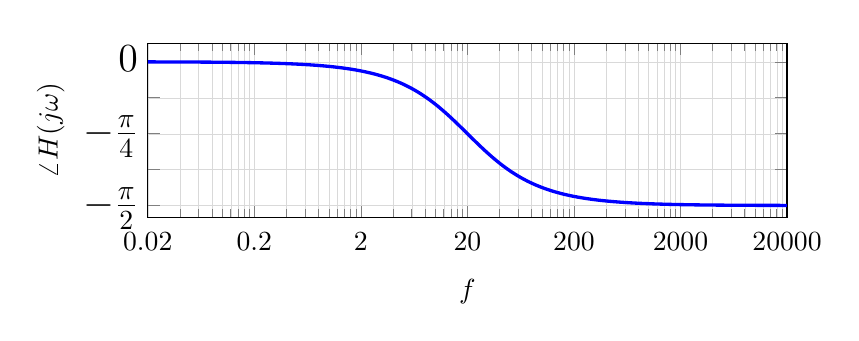
\begin{tikzpicture}[
    declare function={
      phase(\omega) = -rad(atan(\omega / 10^8))
      % Straight line bode approximation
      % phase(\omega)= (\omega < 10^7) * (0) +
      %           and(\omega >= 10^7, \omega < 10^9) * (-pi / 4 * (log10(\omega) - 7)) +
      %           (\omega >= 10^9) * (-pi / 2)
     ;
    }
  ]
  \begin{semilogxaxis}[
    typeset ticklabels with strut,
    ymin= -1.7, ymax=0.2, ylabel=$\angle H(j \omega)$,
    ytick={-pi/2, -3*pi/8, -pi/4, -pi/8, 0},
    yticklabel style={font=\Large},
    yticklabels={$-\frac{\pi}{2}$, $\,$, $-\frac{\pi}{4}$, $\,$, $0$},
    xticklabels={$0.02$,$0.2$,$2$,$20$, $200$, $2000$, $20000$},
    xmin=10^5, xmax=10^11, xlabel=$f$,
    domain=10^5:10^11,
    grid=both, grid style={line width=.1pt, draw=gray!30},
    width=\textwidth * 0.8,
    height=\textwidth / 3.2,
    samples = 600
  ]
    \addplot [blue,very thick] {phase(x)};
  \end{semilogxaxis}
  \end{tikzpicture}
  \end{figure}
  \newpage
  }   

  \qitem Now, let's say that our filter is successful at removing the interference we initially detected. We now notice that there is another source of interference--Delta brainwaves--in the frequency range 0.5Hz to 4Hz. \textbf{How could we modify our design to remove both sources of interference and get a clear recording of Alpha brainwaves?} Suppose you have access to an inductor as well.

  \sol {
  Replace our low-pass filter with a bandpass filter. This will attenuate both sources of noise and leave our frequency band for Alpha brainwaves intact for our sensor to record.

  To design our bandpass, we can use the following cirucuit:

  \begin{center}
  \begin{circuitikz}[scale=0.8]
      \draw (0,4) 
      to [sV, l= $V_s$] (0,0)
      (0,4)
      to [C = $C$] (3,4)
      to [L = $L$,] (6,4)
      to [short] (8,4)
      to [R = $R$] (8,0)  
      to [short] (0,0)
      (8, 4) to[short, -o] (9, 4) node[anchor=west] (+) {+}
      (8, 0) to[short, -o] (9, 0) node[anchor=west] (-) {-}
      (+) to[open, l^=$\widetilde{V}_{\text{out}}$] (-)
      ;
  \end{circuitikz}
\end{center}

  Using previous phasor analysis techniques, we can see this as a voltage divider by taking the capacitor and inductor as one impedance in series.
  $$H(j \omega) = \frac{R}{R + j \omega L + \frac{1}{j \omega C}} = \frac{j \omega RC}{1 + j \omega RC + (j \omega)^{2} LC}$$
  }

  \qitem Ideally, what would we want our cutoff frequencies to be?

  \sol {
    We currently want to capture Alpha brainwaves running at 8 to 13 Hz, while filtering out Gamma brainwaves at 32 to 100 Hz, and Delta brainwaves at 0.5 to 4 Hz. While a low cutoff frequency of 8 and high cutoff frequency of 13 will do the job ideally, we must also account for noise in the Alpha brainwaves. Therefore, we should pick a low frequency in between 4 and 8 Hz, and a high frequency in between 13 and 32 Hz. A low cutoff frequency of 6Hz, and a high cutoff frequency of 22 Hz should do the job.
  }

  \qitem How can we calculate the cutoff frequencies for our filter in terms of R, L, and C? 

  \meta {
    We use $\sqrt{\frac{1}{2}}$ since it is the half power point.
  }

  \sol {
    Remember that in order to find the cutoff frequencies, we find the frequencies at which $|H(j \omega)| = \frac{1}{\sqrt{2}}.$
    $$|H(j \omega)| = \frac{\omega RC}{\sqrt{(1 - \omega^{2} LC)^2 + (\omega RC)^2}} = \frac{1}{\sqrt{2}}$$
    Squaring both sides, we get:
    $$\Big( \frac{\omega RC}{\sqrt{(1 - \omega^{2} LC)^2 + (\omega RC)^2}} \Big)^{2} = \frac{(\omega RC)^2}{(1 - \omega^{2} LC)^2 + (\omega RC)^2} = \frac{1}{2}$$
    Cross multiplying, we get:
    $$(1 - \omega^{2} LC)^2 + (\omega RC)^2 = 2 (\omega RC)^2 \ \ \text{or} \ \ (1 - \omega^{2} LC)^2 = (\omega RC)^2$$
    We take the square root of both sides, and taking the negative case into account,
    $$(1 - \omega^{2} LC) = \pm \omega RC$$
    Now, we can use the quadratic formula twice, and note that we'll have four solutions, but we will only consider the positive valued ones.
    $$\omega = \pm \frac{R}{2L} + \sqrt{\big(\frac{R}{L}\big)^2 + \frac{4}{LC}}$$ 
  }

  \qitem Let's pick values of $R, L,$ and $C$ to pick our cutoff 



\end{enumerate}